\documentclass{article}
\usepackage[utf8]{inputenc}
\usepackage{amsmath}
\usepackage{listings}
\usepackage{graphicx}
\usepackage[shortlabels]{enumitem}

\title{CIS 419/519: Homework 1}
\author{Zitong Zhu}
\date{}

\begin{document}
    \maketitle
    Although the solutions are my own, I consulted with the following people while working on this homework: \{Names here\}

    \begin{enumerate}
        \item % 1
        \begin{enumerate}
            \item % a
            Show your work:
            \begin{equation*}
                P(\textrm{play outside = yes}) = 30/50
            \end{equation*}
            \begin{equation*}
                P(\textrm{play outside = no}) = 20
            \end{equation*}\\
            For Sunny = Yes: \\
            \begin{equation*}
            	P_{Yes}=\frac{25}{31}, P_{No}=\frac{6}{31},\\
            S_{Sunny=Yes}=-\frac{25}{31} log_{2} \frac{25}{31} - \frac{6}{31} log_{2} \frac{6}{31}=0.7554
            \end{equation*}
            For Sunny = No: \\
             \begin{equation*}
            	P_{Yes}=\frac{25}{31}, P_{No}=\frac{6}{31},\\
            S_{Sunny=No}=-\frac{5}{19} log_{2} \frac{5}{19} - \frac{14}{19} log_{2} \frac{14}{19}=0.8315
            \end{equation*}
            For Snow = Yes: \\
             \begin{equation*}
            	P_{Yes}=\frac{14}{18}, P_{No}=\frac{4}{18},\\
            S_{Sunny=Yes}=-\frac{14}{18} log_{2} \frac{14}{18} - \frac{4}{18} log_{2} \frac{4}{18}=0.7642
            \end{equation*}
            For Snow = No: \\
             \begin{equation*}
            	P_{Yes}=\frac{16}{32}, P_{No}=\frac{16}{32},\\
            S_{Sunny=Yes}=-\frac{16}{32} log_{2} \frac{16}{32} - \frac{16}{32} log_{2} \frac{16}{32}=1
            \end{equation*}
            
            \begin{equation*}
                IG_{Snow} = 0.9709-(0.7642*\frac{18}{50}+1*\frac{32}{50})=0.0558
            \end{equation*}
            \begin{equation*}
                IG_{Sunny} = 0.9709-(0.7088*\frac{31}{50}+0.8315*\frac{19}{50})=0.2155
            \end{equation*}
            Sunny is better because it has a larger IG.

            \item % b
            \textbf{For Root:} \\
	\begin{equation*}
	\begin{split}
	MinError for all elements:\\
	Inflated: min(\frac{6}{17}, \frac{11}{17}) = \frac{6}{17}\\
	Color_{Blue}: min(\frac{3}{12}, \frac{9}{12}) = \frac{3}{12}\\
	Color_{Red}: min(\frac{3}{5}, \frac{2}{5}) = \frac{2}{5}\\
	Size_{Large}: min(\frac{5}{8}, \frac{3}{8}) = \frac{3}{8}\\
	Size_{Small}: min(\frac{1}{9}, \frac{8}{9}) = \frac{1}{9}\\
	Act_{Stretch}: min(\frac{5}{9}, \frac{4}{9}) = \frac{4}{9}\\
	Act_{Dip}: min(\frac{1}{8}, \frac{7}{8}) = \frac{1}{8}\\
	Age_{Adult}: min(\frac{1}{6}, \frac{5}{6}) = \frac{1}{6}\\
	Age_{Child}: min(\frac{5}{11}, \frac{6}{11}) = \frac{5}{11}\\
	\end{split}
	\end{equation*}
            Color: 
            \begin{equation*}
            Gain_{ME}(color)=MinError(Inflated)-\frac{12}{17}MinError(Blue)-\frac{5}{17}MinError(Red)\\
             \end{equation*}
              \begin{equation*}
            =\frac{6}{17}-\frac{12}{17} \times \frac{3}{12}-\frac{5}{17} \times \frac{2}{5}\\
            =\frac{1}{17}
            \end{equation*}
            By using the same function, we can get:\\
            $Gain_{ME}(size)=\frac{2}{17}$, \\
            $Gain_{ME}(act)=\frac{1}{17}$,\\
            $Gain_{ME}(age)=0$.\\ 
            Obviously, $Gain_{ME}(size)$ is the largest.\\
   	    Therefore, the first split is on: size.\\\\
            \textbf{For Level 1:}\\
            When size = Large: \\
            \begin{equation*}
            \begin{split}
            MinError for all elements:\\
	Inflated: min(\frac{5}{8}, \frac{3}{8}) = \frac{3}{8}\\
	Color_{Blue}: min(\frac{2}{5}, \frac{3}{5}) = \frac{2}{5}\\
	Color_{Red}: min(\frac{3}{3}, \frac{0}{3}) = 0\\
	Act_{Stretch}: min(\frac{5}{5}, \frac{0}{5}) = 0\\
	Act_{Dip}: min(\frac{0}{3}, \frac{3}{3}) = 0\\
	Age_{Adult}: min(\frac{0}{1}, \frac{1}{1}) = 0\\
	Age_{Child}: min(\frac{5}{7}, \frac{2}{7}) = \frac{2}{7}\\
	\end{split}
	\end{equation*}
            $Gain_{ME}(color)=\frac{1}{8}$,\\
            $Gain_{ME}(act)=\frac{3}{8}$,\\
            $Gain_{ME}(age)=\frac{1}{8}$.\\
            Obviously,$Gain_{ME}(act) $is the largest.\\
            Therefore, the second split when size is large is on act. The inflated only depends on act here.\\
            When size = Small: \\
         \begin{equation*}
	\begin{split}
	MinError for all elements:\\
	Inflated: min(\frac{1}{9}, \frac{8}{9}) = \frac{1}{9}\\
	Color_{Blue}: min(\frac{1}{7}, \frac{6}{7}) = \frac{1}{7}\\
	Color_{Red}: min(\frac{0}{2}, \frac{2}{2}) = 0\\
	Act_{Stretch}: min(\frac{0}{4}, \frac{4}{4}) = 0\\
	Act_{Dip}: min(\frac{1}{5}, \frac{4}{5}) = \frac{1}{5}\\
	Age_{Adult}: min(\frac{1}{5}, \frac{4}{5}) = \frac{1}{5}\\
	Age_{Child}: min(\frac{0}{4}, \frac{4}{4}) = 0\\
	\end{split}
	\end{equation*}
            $Gain_{ME}(color)=0$, \\
            $Gain_{ME}(act)=0$, \\
            $Gain_{ME}(age)=0$. \\
            Since they all equal, choose the first one: color.\\
            Therefore, the second split when size is small is on color.\\\\
            \textbf{For Level-2}:\\
            When color = Red, the inflated is all False.\\
            When color = Blue, \\
            \begin{equation*}
            \begin{split}
            MinError for all elements:\\
	Inflated: min(\frac{1}{7}, \frac{6}{1}) = \frac{1}{7}\\
	Act_{Stretch}: min(\frac{0}{4}, \frac{4}{4}) = 0\\
	Act_{Dip}: min(\frac{1}{3}, \frac{2}{3}) = \frac{1}{3}\\
	Age_{Adult}: min(\frac{1}{5}, \frac{4}{5}) = \frac{1}{5}\\
	Age_{Child}: min(\frac{0}{2}, \frac{2}{2}) = 0\\
	\end{split}
	\end{equation*}
            $Gain_{ME}(act)=0$, \\
            $Gain_{ME}(age)=0$. \\
            Since they all equal, choose the first one: act.\\
            Therefore, the third split when color is blue is on act.\\\\
            \textbf{For Level-3}:\\
            When act = Stretch, the inflated is all False.\\
            When act = Dip, it depends on Age, and if age=Adult, the inflated is True, if age=Child, the inflated is False.\\
            \\The Decision Tree that made by ID3 Algorithm is below:\\

            % The template tree is meaningless (it's not a hint about what the answer is)
            \begin{verbatim}
                if size = Large:
                  if act = Stretch:
                    inflated = T
                  if act = Dip:
                    inflated = F
                if size = Small:
                  if color = Blue:
                    if act = Stretch:
                      inflated = F
                    if act = Dip:
                      if age = Adult:
                        inflated = T
                      if age = Child:
                       inflated = F
                  if color = Red:
                    inflated = F
            \end{verbatim}

            \item % c
            No because ID3 algorithm is only focus on the local optimization which only chooses the optimal choice under one root (split). It cannot guarantee the choice is optimal for the global tree. For example, for question 1b, on the split of size=small, the optimal choice is splitting on age or act then the depth will be minimum depth, but it split on color which depth is larger because for that root all the three have the same IG.
        \end{enumerate}

        \item % 2
        \begin{enumerate}
            \item % (a)
            See Figure~\ref{fig:model_performance} for the model performance in the Madelon dataset.
            \begin{figure}
                \centering
                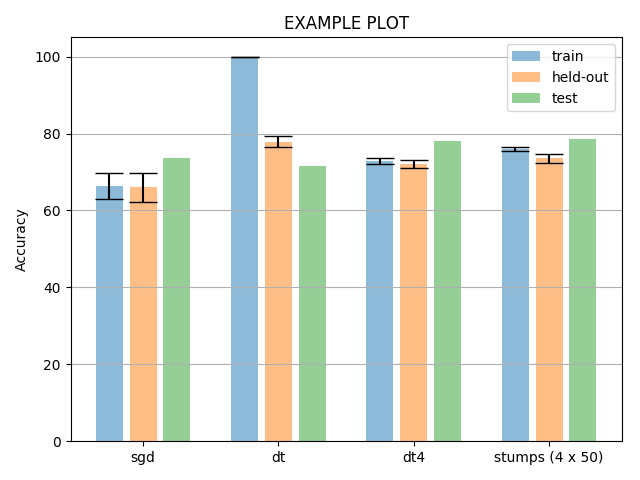
\includegraphics[width=\textwidth]{plot.png}
                \caption{Model performance on the Madelon dataset}
                \label{fig:model_performance}
            \end{figure}
	
            \begin{enumerate}[1.]
                \item $Stumps_{heldout} > DT4_{heldout} > DT_{heldout} > SGD_{heldout}$\\
                		$Stumps_{test} > DT4_{test} > DT_{test} > SGD_{test}$\\
			The order for heldout and test is the same. Stumps is the best, and SGD is the worst.\\
			$acc_{heldout}$ is similar to $acc_{test}$.\\
                \item Decision Tree has the highest train accuracy since there is no limit of the depth, so it is over-fitting for the data. Hence, all the train can be predict right.
                \item 
		The confidence intervals calculated for each model are as following
		\begin{center}
                \begin{tabular}{|c|c|c|}
                    \hline Algorithm &Confidence Interval$_{train}$ & Confidence Interval$_{heldout}$ \\
                    \hline SGD & (0.592, 0.763) & (0.521, 0.544) \\
                    Decision Tree & (1.0, 1.0) & (0.732, 0.796) \\
                    Decision Stump & (0.767, 0.799) & (0.741, 0.788) \\
                    SGD + Decision Stump Features & (0.856, 0.884) & (0.787, 0.817) \\ \hline
                \end{tabular}
            \end{center}
            No. It is obviously that only SGD is statistically significant since there is no overlap. To deal with that, increase the number of fold cross-validation, so the number of accuracies will increase, 
            then the mean will be closer to the real accuracy of the model. As a result, the std becomes less and has a tight confidence interval.
                \item
                Cross-Validation can remove the affect which caused by special cases of data. Each element in the train set was considered as both train set and test set, 
                so it is more reliable than only test on one test and train set. It is also closer to the real accuracy since there are more accuracies from the same model.  In addition, cross validation produces some other data, such as confidence interval, c
                an be used to evaluate the model in other ways more than only focus on accuracy.
            \end{enumerate}

            \item % (b)
            The models' accuracies on the Badges dataset were as follows:
            \begin{center}
                \begin{tabular}{|c|c|c|}
                    \hline Algorithm & Accuracy$_{train}$ & Accuracy$_{test}$ \\
                    \hline SGD & 0.765 & 0.625 \\
                    Decision Tree & 1.0 & 0.62 \\
                    Decision Stump & 0.677 & 0.650 \\
                    SGD + Decision Stump Features & 0.742 & 0.656 \\ \hline
                \end{tabular}
                 \begin{tabular}{|c|c|c|}
                    \hline Algorithm & Accuracy$_{train}$ & Accuracy$_{test}$ \\
                    \hline SGD & 0.766 & 0.625 \\
                    Decision Tree & 1.0 & 0.612 \\
                    Decision Stump & 0.677 & 0.65 \\
                    SGD + Decision Stump Features & 0.741 & 0.637 \\ \hline
                \end{tabular}
            \end{center}

            \begin{enumerate}[1.]
                \item 
                For train set, the rank is always:\\
                $DT_{train} > SGD_{train} > Stump_{train} > DT4_{train}$\\
                However, for test set, the rank is not constant. It can be: 
                $DT4_{test} > Stump_{test} > SGD_{test} > DT_{test}$\\
                OR\\
                $Stump_{test} > DT4_{test} > SGD_{test} > DT_{test}$\\
                It can be said that Stump is both the best in Medelon and Badges. Although it may not be the highest accuracy sometimes, it is really close to DT4.
            \end{enumerate}

            \textbf{Extra Credit}:\\
             I checked the first 15 characters of first name and last name to see if it is a vowel. If it is, set feature = 1, otherwise = 0. Then use Decision Tree Classifier to train the model
             since the features are specific and Decision Tree can fit features well. The accuracy that I got is almost 84\% so I believe it is a good features choice.
             
        \end{enumerate}
    \end{enumerate}
\end{document}
